\section{Evaluation}\label{sec:evaluation}

\subsection{What Worked Before Review Stage}
In the mid report, we swept nx from 100 to 500 to see how the performance works given $nx$. First, like we have mentioned above, we could see timing is proportional to $ nx^{3} $. In terms of performance improvement, we could achieve quite good improvement by just doing vectorization. If you see Figure ~\ref{fig:vector_timing_result1}, vectorization did more jobs per second. 

We evaluate our different simulators using our own timing plots. Timing result with vectorization can be found at Figure ~\ref{fig:vector_timing_result1} and Figure ~\ref{fig:vector_timing_result2}. In Figure ~\ref{fig:vector_timing_result1}, we plot cells/seconds vs. $nx$. We used the cube of cells. As discussed in Piazza (Referring to Prof. Bindel's answer), there are two important factors: the time between frames, and the time step. Total time is proportional to $ nx^{3} $. In Figure ~\ref{fig:vector_timing_result2}, we can clearly see timing is proportional to $ nx^{3} $. Note that "copy" is our initial result from the very first scratch (i.e. no modification), and "vec" indicates our vectorization result.

\begin{figure}[h]
    \centering
    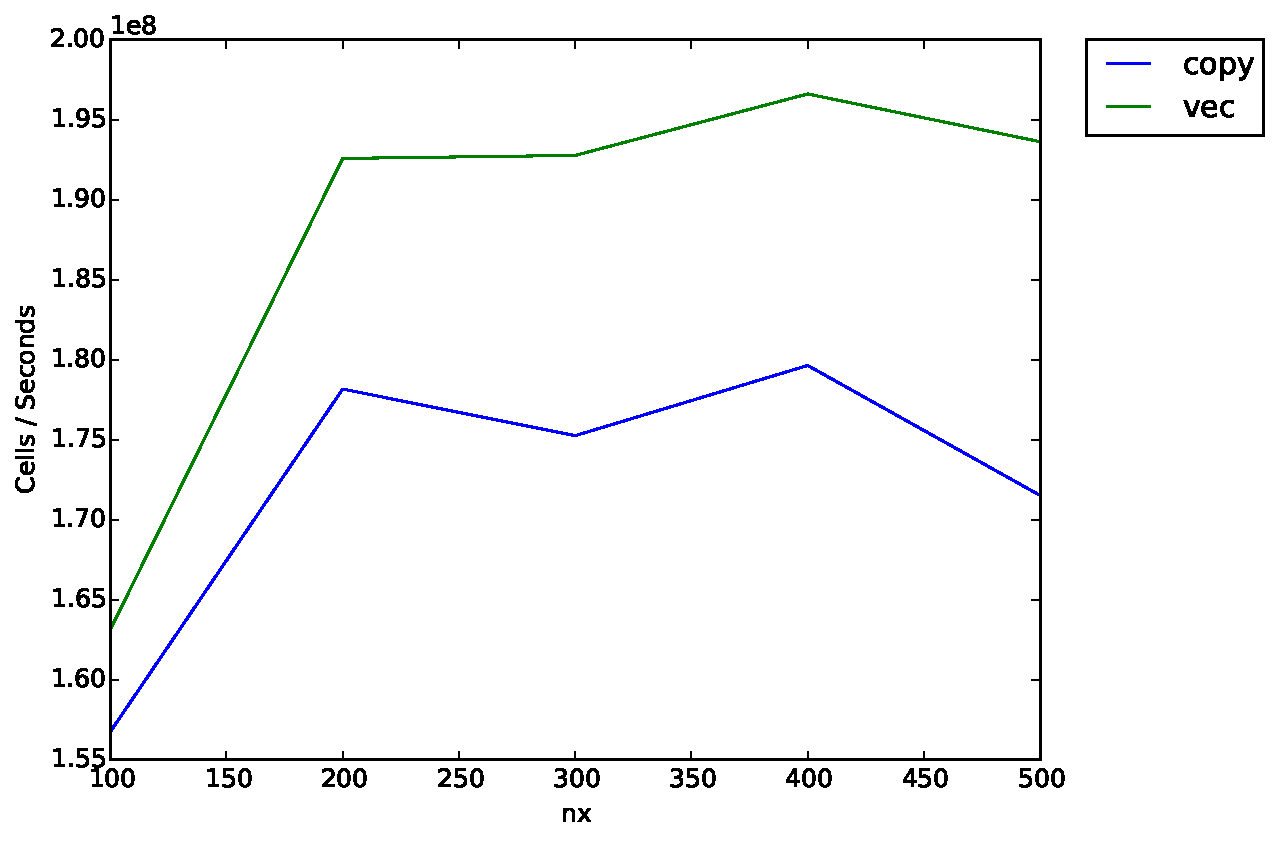
\includegraphics[width=0.8\textwidth]{figs/vec-timing1.pdf}
    \caption{Vector Timing Result - Mid result ($cells/seconds$ vs. $nx$)}
    \label{fig:vector_timing_result1}
\end{figure}

\begin{figure}[h]
    \centering
    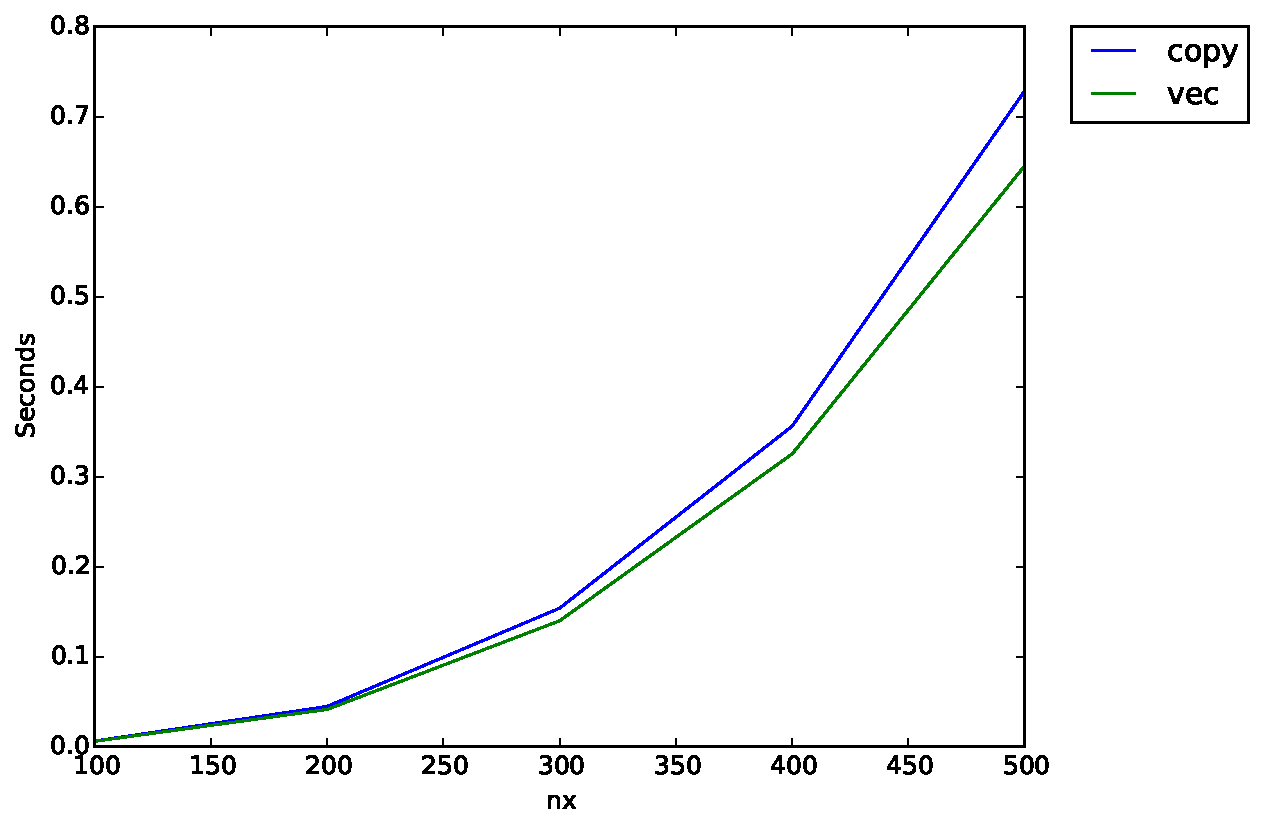
\includegraphics[width=0.8\textwidth]{figs/vec-timing2.pdf}
    \caption{Vector Timing Result - Mid result  ($seconds$ vs. $nx$)}
    \label{fig:vector_timing_result2}
\end{figure}

\subsection{What Did Not Work Before Review Stage}
We tried OpenMP to make it parallel. Like we said at earlier section, OpenMP is a powerful tool to use to increase performance, but we noticed that it actually decreases the performance. Since it exceeded wall clock time, we could not even get the result yet.

\subsection{What Worked After Review Stage}
After the review stages, we further tried blocking and domain decomposition, while keep improving our vectorization and OpenMP stuffs.

This time, we swept $ nx $ from 500 to 1500 to check our performance with reasonable size of $ nx $. See
Figure ~\ref{fig:final_timing_result1} and Figure ~\ref{fig:final_timing_result2}. Here, "shallow" is the initial version, while "opt" indicates our final optimized version. 

Based on our qualitative and quantitative evaluations, we could see that our
optimal version was able to spread computation very well over the clusters. We were able to improve the performance only with blocking or only with vectorization. By exploiting vectorization and blocking all together, howver, performance can be even more improved than before. In our experiments, the performance got improved by 7-8x in average and up to 10x when $ nx $ is 700. We expect this can be even higher, as we tuned our design more, but we firmly believe that 10x improvement is still good to see. In minor, we found that the performance is sometimes degraded when $ nx $ is too small.  

\begin{figure}[h]
    \centering
    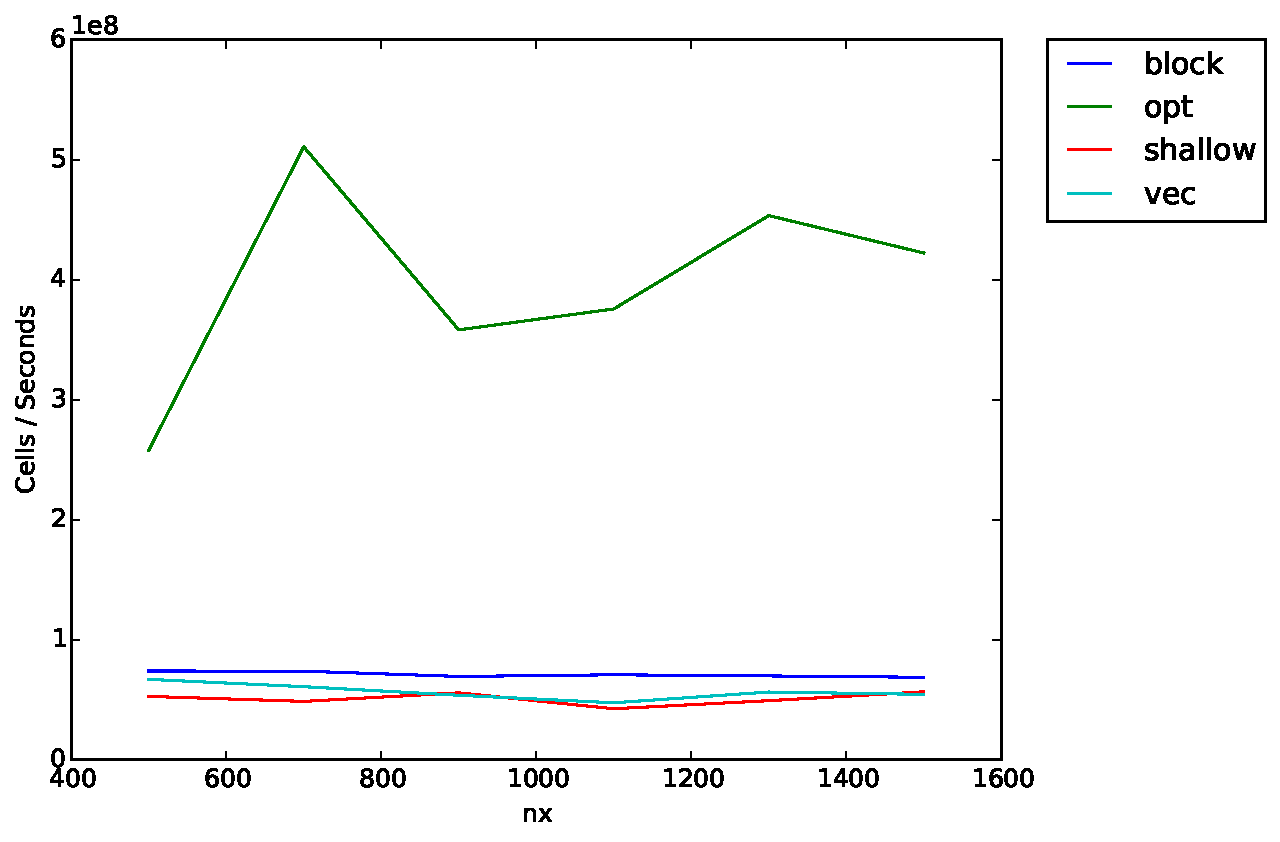
\includegraphics[width=0.8\textwidth]{figs/final-timing1.pdf}
    \caption{Final Timing Result ($cells/seconds$ vs. $nx$)}
    \label{fig:final_timing_result1}
\end{figure}

\begin{figure}[h]
    \centering
    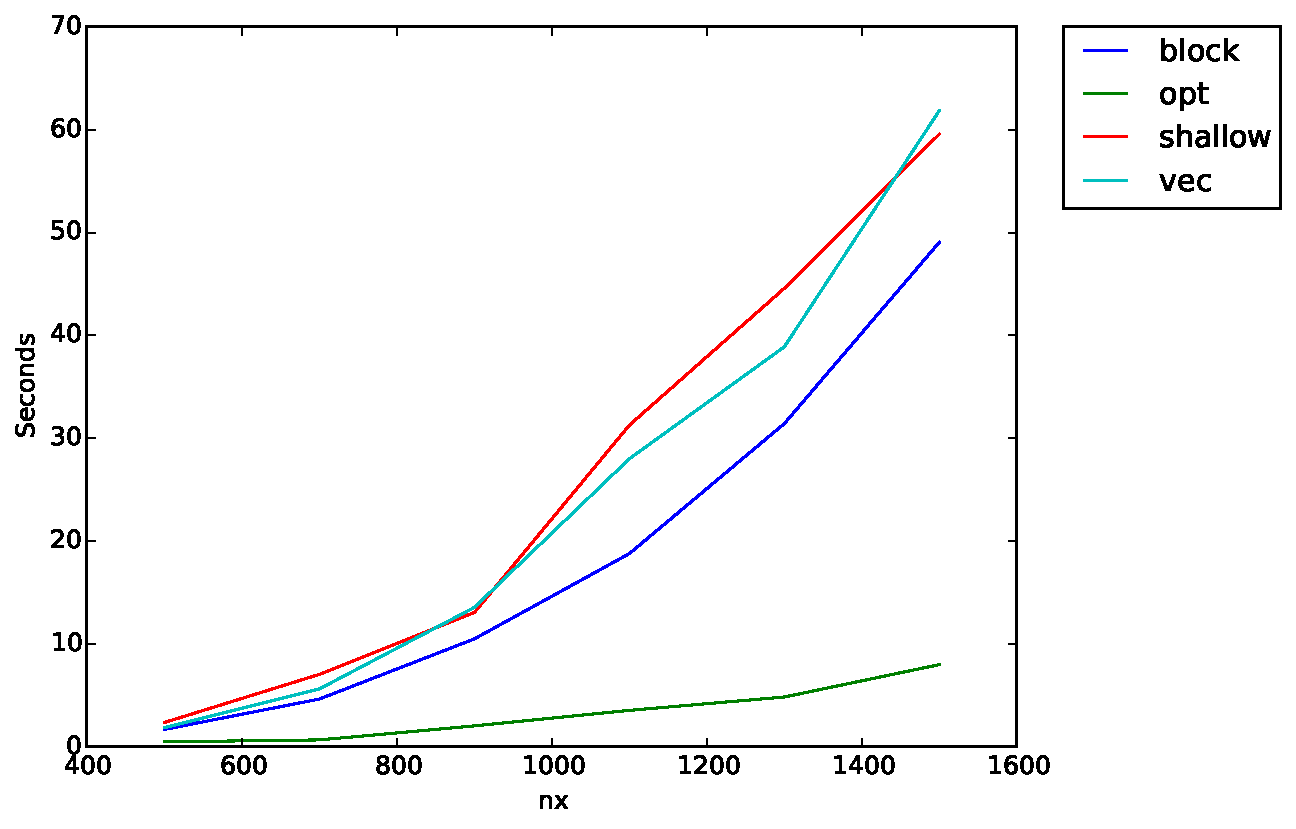
\includegraphics[width=0.8\textwidth]{figs/final-timing2.pdf}
    \caption{Final Timing Result ($seconds$ vs. $nx$)}
    \label{fig:final_timing_result2}
\end{figure}

